\hypertarget{abstract}{%
\section{Abstract}\label{abstract}}

Invariant-aware validators can outperform structural baselines on
constructed errors without establishing their performance on
independently labeled records. We examine this distinction in two finite
synthetic validation designs and a failed external-fixture attempt. The
invariant-aware method has balanced accuracy 1, while the baseline has
0.5 and 0.5980. A separate, protocol-locked exploratory audit recomputes
195 overall split/method metric comparisons from frozen prediction
artifacts; all agree within declared serialization tolerances. Exact
finite score-group Brier decomposition shows that improved resolution
accounts for lower Brier scores even as empirical reliability worsens. A
binary-probability ablation has zero Brier score and zero expected
calibration error with unchanged decisions. We find one distinct
cluster-statistic signature among 64 evaluation clusters in the first
design and six among 48 in the second. These counts describe limits of
the resampling evidence without estimating effective sample size.
Conditional arguments connect perfect finite agreement, Laplace
smoothing and degenerate resampling to test construction. The
contribution is an auditable methods case study, rather than a new
validator or evidence of production accuracy.

\hypertarget{introduction}{%
\section{1. Introduction}\label{introduction}}

A structural validator may verify required fields and primitive types,
while an invariant checker may also compare identities, conservation
relations or state transitions. A benchmark that injects violations of
the additional relations will often favor the invariant-aware method.
The scientific question is what that comparison establishes beyond
correct handling of the selected construction.

We examine our own benchmark artifacts, rather than an unrelated
deployed system. The initial comparison produced large improvements and
perfect invariant-aware decisions. However, benchmark truth, fault
inventory and validator were developed under closely related
specifications. Probability-score improvements were also easy to
overinterpret: lower Brier scores appeared alongside higher expected
calibration error (ECE). An attempted extension to public event fixtures
later stopped before evaluation because its source contract rejected
repeated IDs.

We ask three questions. RQ1: do separately recomputed metrics and
alignment checks support the reported finite comparisons? RQ2: which
components explain the probability-score changes? RQ3: what do repeated
cluster statistics and the external source failure imply about the scope
of evidence?

The contribution combines a traceable case study, a standalone artifact
audit and conditional explanations of the observed behavior. Invariant
checking, the oracle problem, Brier decomposition and calibration
caveats are established ideas. We do not present them as new. The
empirical contribution is their application to these particular
versioned constructions, including the negative calibration finding and
preservation of an invalid external attempt.

\hypertarget{related-work-and-position}{%
\section{2. Related work and position}\label{related-work-and-position}}

Schelter et al.~{[}1{]} combine declarative data-quality constraints
with user-defined checks and scalable execution. Breck et al.~{[}2{]}
study validation for machine-learning data pipelines. Practical
validation thus extends beyond primitive record shapes; our narrow
structural baseline does not represent all schema languages or
data-quality systems. We make no comparative performance claim against
these systems.

Barr et al.~{[}3{]} examine the difficulty of deciding whether observed
software behavior is correct. Our case illustrates a related
distinction: separate implementations of an oracle and checker reduce
shared-code risk while potentially retaining a shared specification.
Agreement does not establish that this specification captures an
external task.

Murphy {[}4{]} separates probability-score behavior into reliability,
resolution and uncertainty. We use an exact finite binary score-group
form and provide its algebra below. Guo et al.~{[}5{]} study confidence
calibration; Nixon et al.~{[}6{]} examine how calibration-measure
choices affect conclusions. Our validators are deterministic rule
systems, not neural networks. These sources ground measurement
terminology rather than supply evidence about our methods. Our ECE
compares positive-class probability with observed positive frequency,
not maximum-class confidence with classification correctness.

This is a focused comparison with relevant foundations, not a systematic
literature review. The case documents an instance of known measurement
concerns, with arithmetic that can be checked from frozen rows. It does
not establish a new general limitation of validation systems.

\hypertarget{designs-and-evidence-status}{%
\section{3. Designs and evidence
status}\label{designs-and-evidence-status}}

\hypertarget{methods-and-positive-class}{%
\subsection{3.1. Methods and positive
class}\label{methods-and-positive-class}}

The positive class is \textbf{valid}. A false positive is an invalid
case accepted; a false negative is a valid case rejected. We use

\[
\mathrm{BA}=\tfrac12\left(\frac{TP}{TP+FN}+\frac{TN}{TN+FP}\right),\quad
\mathrm{FPR}=\frac{FP}{TN+FP},\quad \mathrm{FNR}=\frac{FN}{TP+FN}.
\]

B0 applies each protocol's structural rules. M1 adds its selected
semantic and state relations. The no-semantic and no-state ablations
remove the corresponding predicates. The no-calibration ablation
preserves M1's decisions and reports each binary decision as its
probability. B0 is deliberately limited; the study does not show that
relational validation is impossible with richer schemas or existing
constraint systems.

Each calibrated method fits a calibration-only lookup on raw score
\(s\):

\[
\widehat p(y=1\mid s)=\frac{k_s+1}{n_s+2},
\]

where \(n_s\) is the calibration score-group size and \(k_s\) its
positive count. An unseen score uses the formula on all calibration
cases. This is Laplace-smoothed empirical lookup, not isotonic
regression. It does not change classification decisions.

\hypertarget{synthetic-constructions}{%
\subsection{3.2. Synthetic
constructions}\label{synthetic-constructions}}

E001 creates entity, ledger and event bundles with identity,
conservation, transition-legality and revision-consistency relations.
Its complete synthetic oracle is coupled to its recipes. E002 adds six
heterogeneous cluster types, bounded multiple-fault recipes and a
separately implemented replay/conservation oracle. Omitted conservation,
overconstraints and stale transitions are deliberate specification
stressors.

\noindent\begin{minipage}{\linewidth}
\noindent Table 1. Original case counts and evaluation clusters. Clusters group
related cases from one constructed base or template instance.
\par\medskip\centering
\begin{tabular}{@{}lrrrr@{}}
\toprule
Design & Development & Calibration & Evaluation & Evaluation clusters \\
\midrule

E001 & 256 & 256 & 512 & 64 \\
E002 & 228 & 228 & 456 & 48 \\
\bottomrule
\end{tabular}
\end{minipage}


The evaluation split is historically named \texttt{confirmatory}.
Original protocols were locked before their valid runs. E005, the audit
in this paper, was locked after those results had been inspected and is
explicitly exploratory. It does not create an untouched replication.
E002's earlier invalid run is excluded; its valid run followed a
report-validator correction preserved in the repository.

\hypertarget{external-sources}{%
\subsection{3.3. External sources}\label{external-sources}}

E003-v1 selected three fixed GH Archive hourly files {[}7{]}, with
67,145, 90,940 and 117,780 records. It planned oracle-filtered clean
bases and artificial mutations. Even success would not estimate
naturally occurring error prevalence. The run stopped on repeated event
IDs in the 2021 file before generating predictions or performance
metrics. It supplies no external hypothesis outcome.

A separately locked E004 diagnostic found 537 extra occurrences in 537
groups of size two. Every extra occurrence matched its first raw line
byte for byte, excluding line endings. No conflicting repeated-ID group
or cross-file repeated ID was found in these files. The cause of the
duplicates is unknown. E003-v2's revised policy is informed by those
observations and remains unexecuted; reused sources cannot become a
pristine holdout by renaming a split. We retain the failed attempt as a
limitation.

\hypertarget{exploratory-audit-protocol}{%
\section{4. Exploratory audit
protocol}\label{exploratory-audit-protocol}}

E005-v1 was committed before implementation and one data execution. Its
four immutable inputs contain 5,120 E001 and 7,296 E002 prediction rows,
plus 75 and 243 metric rows. SHA-256 pins are verified before parsing.
The audit imports neither original metric implementation and does not
rerun the old experiments or bootstraps.

Serialized probabilities are parsed as exact decimal rationals. The
audit rejects duplicate JSON or case/method keys, invalid types,
incomplete method coverage, and per-case disagreement in truth, input
hash or cluster identity. It checks split disjointness of bases/clusters
and counts cross-split input-hash overlap. None was found here; that
does not exclude every form of leakage.

Every overall split/method row is checked. Confusion counts must agree
exactly; absolute metric tolerances are \(10^{-9}\) for E001 and
\(2\times10^{-9}\) for E002, allowing serialization and displayed
rounding. ECE uses ten equal-width bins, lower bound included and upper
bound excluded, except that the final bin includes 1:

\[
\mathrm{ECE}_{10}=\sum_{b=0}^{9}\frac{N_b}{N}|\overline p_b-\overline y_b|.
\]

The audit reconstructs lookups using calibration rows only and checks
every stored probability. Success establishes compatibility with that
rule, not historical proof of which rows were used during fitting.
Binary-ablation probabilities must equal decisions exactly.

For each distinct serialized probability \(p_g\), let \(w_g=N_g/N\) and
let \(f_g\) be its group's observed positive frequency. With overall
frequency \(\bar y\),

\[
\begin{aligned}
\mathrm{REL}&=\sum_g w_g(p_g-f_g)^2, &
\mathrm{RES}&=\sum_g w_g(f_g-\bar y)^2,\\
\mathrm{UNC}&=\bar y(1-\bar y), &
\mathrm{BS}&=\mathrm{REL}-\mathrm{RES}+\mathrm{UNC}.
\end{aligned}
\]

These are exact score groups, not ECE bins. Within-group mean squared
error is \((p_g-f_g)^2+f_g(1-f_g)\). Weighted outcome variances satisfy

\[
\sum_g w_g f_g(1-f_g)=\bar y(1-\bar y)-\sum_g w_g(f_g-\bar y)^2.
\]

Substitution proves the stated binary Brier identity. The audit requires
zero rational residual. This finite-sample identity does not make REL a
consistent population-calibration estimate in arbitrary small or
singleton groups.

For each method, we also count distinct cluster-statistic signatures:
TP/TN/FP/FN, summed squared probability error, and each ECE bin's count,
probability sum and truth sum. IDs and row order are omitted. This
diagnoses statistic diversity and does not estimate effective sample
size.

The implementation passed 21 synthetic tests, covering mixed-label score
groups, bin boundaries, lookup fallback, rounding and late write
failures. All four outputs are built twice and compared byte for byte
before the report is published last. Tests and the separate
implementation share an author and environment; independent scientific
acceptance remains absent.

\hypertarget{results}{%
\section{5. Results}\label{results}}

\hypertarget{metric-agreement-and-finite-performance}{%
\subsection{5.1. Metric agreement and finite
performance}\label{metric-agreement-and-finite-performance}}

All 195 overall split/method metric comparisons pass. Maximum absolute
differences from frozen CSV values are \(1.013\times10^{-15}\) for E001
and \(4.706\times10^{-10}\) for E002. Confusion counts agree exactly.
Alignment, split disjointness and lookup-compatibility checks pass.
Every one of the 39 split/method rows satisfies the Brier identity
exactly.

\noindent\begin{minipage}{\linewidth}
\noindent Table 2. Evaluation metrics recomputed from frozen rows. Binary is the
no-calibration ablation with unchanged decisions.
\par\medskip\centering
\begin{tabular}{@{}llrrrrr@{}}
\toprule
Design & Method & BA & FPR & FNR & Brier & ECE \\
\midrule

E001 & B0 & 0.500000 & 1.000000 & 0 & 0.25000000 & 0 \\
E001 & M1 & 1.000000 & 0 & 0 & 0.00005917 & 0.00769231 \\
E001 & Binary & 1.000000 & 0 & 0 & 0 & 0 \\
E002 & B0 & 0.598039 & 0.803922 & 0 & 0.09193743 & 0.00740887 \\
E002 & M1 & 1.000000 & 0 & 0 & 0.00024790 & 0.01263163 \\
E002 & Binary & 1.000000 & 0 & 0 & 0 & 0 \\
\bottomrule
\end{tabular}
\end{minipage}


The original 10,000-replicate paired cluster bootstrap gives E001 point
intervals for BA difference 0.5 and FPR difference -1. E002 intervals
are {[}0.383254717, 0.422077922{]} for BA difference and
{[}-0.844327177, -0.767281106{]} for FPR difference. FNR difference is
zero in both designs. These are original finite-design intervals, not
new E005 estimates for a sampled deployment population.

In E002, omitted conservation yields FPR 0.117647; overconstraint and
stale-transition checkers each yield FNR 0.833333. These bounded
failures expose dependence on the selected contract. They do not
establish robustness to arbitrary incorrect specifications.

\hypertarget{resolution-explains-lower-brier}{%
\subsection{5.2. Resolution explains lower
Brier}\label{resolution-explains-lower-brier}}

\noindent\begin{minipage}{\linewidth}
\noindent Table 3. Exact-score decomposition on evaluation rows. Lower REL
indicates lower empirical group reliability loss; higher RES
distinguishes groups with different outcome frequencies. Display
rounding can obscure the exact identity.
\par\medskip\centering
\begin{tabular}{@{}llrrrr@{}}
\toprule
Design & Method & REL & RES & UNC & Brier \\
\midrule

E001 & B0 & 0 & 0 & 0.250000000 & 0.250000000 \\
E001 & M1 & 0.000059172 & 0.250000000 & 0.250000000 & 0.000059172 \\
E002 & B0 & 0.000112121 & 0.002357518 & 0.094182825 & 0.091937429 \\
E002 & M1 & 0.000247903 & 0.094182825 & 0.094182825 & 0.000247903 \\
\bottomrule
\end{tabular}
\end{minipage}


E001 B0 reports 0.5 on a balanced evaluation set: ECE and REL are zero
but resolution is absent. M1 separates labels perfectly, increasing RES
to 0.25. Smoothed probabilities remain inside the endpoints, giving
positive REL. The resolution increase dominates the Brier change.

In E002, RES increases by approximately 0.091825308 and REL by
0.000135781. The net Brier change is approximately -0.091689527. Lower
Brier therefore coexists with worse empirical score-group reliability
and higher ten-bin ECE. This is a result about these rows, not
population calibration.

\begin{figure}
\centering
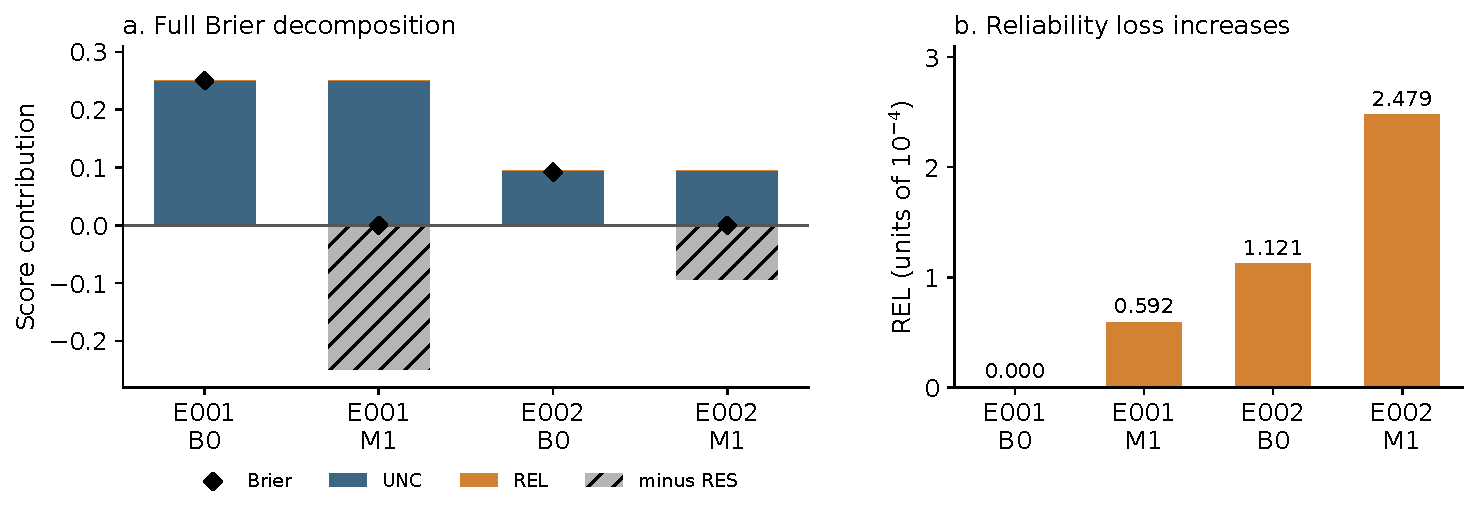
\includegraphics[width=\linewidth]{images/brier-decomposition.pdf}
\caption{Evaluation Brier decomposition: bars show REL, minus RES and
UNC; dots mark their sum, the Brier score. A separate reliability panel
reveals its small increases. Source: E005-v1-summary.csv, evaluation
rows.}
\end{figure}

\hypertarget{statistic-diversity-and-uncertainty}{%
\subsection{5.3. Statistic diversity and
uncertainty}\label{statistic-diversity-and-uncertainty}}

For every method, E001 has one distinct signature among 64 evaluation
clusters. Every bootstrap draw therefore repeats the same vector in the
same number of clusters. More replicates cannot introduce variation
absent from the resampling units.

E002 has six signatures among 48 clusters for every method. Variation in
baseline behavior permits nondegenerate paired intervals, while perfect
M1 decisions persist across its constructed fault inventory. Six
signatures alone do not imply six independent observations or an
effective sample size of six.

\hypertarget{conditional-explanations-and-falsification}{%
\section{6. Conditional explanations and
falsification}\label{conditional-explanations-and-falsification}}

\hypertarget{agreement-on-constructed-support}{%
\subsection{6.1. Agreement on constructed
support}\label{agreement-on-constructed-support}}

Let \(S\) be finite evaluated support with oracle labels \(O(x)\). If
checker \(V\) agrees with \(O\) on every \(x\in S\), and both labels
occur, then FP=FN=0 and BA=1 on \(S\). This follows directly from the
confusion definitions and makes no statement about \(x\notin S\).

When one specification supplies labels and injected violations, perfect
agreement may show conformance to that construction without validating
the specification against external truth. This is conditional: separate
oracle code does not force perfect agreement, and either implementation
could be wrong. Our empirical result is rowwise agreement; attributing
its limited external reach to shared design is an interpretation.
Independently supplied labels exposing disagreements would falsify an
extension of agreement beyond \(S\).

\hypertarget{smoothing-a-perfect-binary-predictor}{%
\subsection{6.2. Smoothing a perfect binary
predictor}\label{smoothing-a-perfect-binary-predictor}}

Suppose each raw-score group has a common label in both calibration and
evaluation. With \(n_g\) calibration cases, smoothing predicts
\(1/(n_g+2)\) or \(1-1/(n_g+2)\). Each evaluation error is then
\(1/(n_g+2)^2\), while the perfect binary predictor has zero error:

\[
\mathrm{BS}_{\mathrm{smooth}}=
\sum_g\frac{N_g^{\mathrm{eval}}}{N^{\mathrm{eval}}}\frac{1}{(n_g+2)^2}>0.
\]

If each ECE bin combines only groups whose errors have the same sign,
ECE is the corresponding weighted average of \(1/(n_g+2)\). These
formulas concern lookup probabilities before serialization; the audit
checks stored decimals within declared tolerances. The observed pure M1
probability groups exhibit this pattern. It does not show that smoothing
is harmful under noise, score overlap, sampling uncertainty or
deployment shift. Hard probabilities are not justified without knowledge
that agreement continues outside the evaluated support.

\hypertarget{repeated-cluster-resampling}{%
\subsection{6.3. Repeated-cluster
resampling}\label{repeated-cluster-resampling}}

If all clusters have the same sufficient-statistic vector, drawing the
original number of clusters always gives the same sum. Any statistic
computed solely from that sum is constant. This explains E001's
degenerate intervals without implying that deployment error is known. A
distinct vector changing the aggregate would falsify this explanation;
none occurs in the locked E005 measurement.

\hypertarget{threats-to-validity-and-implications}{%
\section{7. Threats to validity and
implications}\label{threats-to-validity-and-implications}}

Only two hand-designed benchmark families are analyzed. They are not
randomly sampled tasks, validators or error mechanisms. E001 truth is
recipe-coupled; E002's separate oracle shares its specified world with
M1. E005 questions were motivated by already inspected results. Locking
E005 prevents subsequent protocol adjustment but cannot remove this
exploratory selection.

Exact arithmetic addresses numerical agreement, not specification
correctness or independent review. One author can reproduce a conceptual
error in multiple implementations. Hashes establish identity and lookup
reconstruction establishes compatibility; neither proves universal
absence of leakage or historical fitting order.

REL can misleadingly suggest calibration quality in small score groups;
ECE can hide within-bin heterogeneity. Their direction agrees here but
both limitations remain. Class balance and selected corruption mix shape
the results. Original intervals are conditional on synthetic
constructions, not a deployment population.

External provenance also does not supply independent labels.
Oracle-filtering public records and injecting known violations remains a
controlled-error evaluation. Stronger transfer evidence requires
independently justified labels and a protocol preserving selection
effects and failures. The invalid E003 attempt and its source diagnostic
do not provide that evidence.

The practical implication is to report decision errors, score
components, specification dependence and resampling diversity together.
These are interpretive checks, not universal numeric acceptance
thresholds. A wider study of independent labels and additional validator
families would be needed to establish how common these effects are.

\hypertarget{conclusion}{%
\section{8. Conclusion}\label{conclusion}}

The finite B0/M1 differences survive a separate metric reimplementation.
Their interpretation changes when score and resampling structure are
explicit: higher resolution explains lower Brier while empirical
reliability and ECE worsen; repeated statistics explain degenerate
intervals. Perfect classification remains evidence of agreement on
selected support. The case supports a bounded audit of benchmark
evidence and leaves performance against independently labeled external
records unresolved.

\hypertarget{reproducibility-and-provenance}{%
\section{Reproducibility and
provenance}\label{reproducibility-and-provenance}}

The local companion artifact preserves original predictions, metrics,
protocols and valid result records. E005 protocol commit is
\texttt{2e6f7c2ec236ebce2bf72f3a026b2ea6de3a80e1}; implementation commit
is \texttt{167f721565d68cc80b54340a3533e3b414deedd8}; result and bounded
computational verification are recorded at \texttt{8692937} and
milestone M18. It produces 39 summary rows, 12 score groups and a JSON
check record with 195 signed differences and input identities.

Use a separate checkout at the implementation commit and run
\path|python3 experiments/E005-benchmark-evidence-audit/code/audit.py|.
It uses the standard library, checks pinned inputs, compares two full
builds and refuses existing outputs. The figure derives from the audit
summary; no raw GH Archive payload is included. Independent assessment,
owner-reviewed author metadata and public release of the new analysis
remain pending.

\hypertarget{use-of-generative-ai}{%
\section{Use of generative AI}\label{use-of-generative-ai}}

Generative AI tools were used substantially for research planning, code
implementation, audit analysis and manuscript drafting. The original
harnesses and the separate metric audit share AI authorship and an
environment; agreement is not independent human validation. This working
draft still requires responsible human author review before submission.

\hypertarget{references}{%
\section{References}\label{references}}

\begin{enumerate}
\def\labelenumi{\arabic{enumi}.}
\tightlist
\item
  Sebastian Schelter, Dustin Lange, Philipp Schmidt, Meltem Celikel,
  Felix Biessmann and Andreas Grafberger. 2018. \emph{Automating
  Large-Scale Data Quality Verification}. PVLDB 11(12), 1781-1794. DOI:
  10.14778/3229863.3229867.
  \href{https://www.vldb.org/pvldb/vol11/p1781-schelter.pdf}{Publisher
  paper}.
\item
  Eric Breck, Marty Zinkevich, Neoklis Polyzotis, Steven Whang and Sudip
  Roy. 2019. \emph{Data Validation for Machine Learning}. Proceedings of
  SysML.
  \href{https://research.google/pubs/data-validation-for-machine-learning/}{Author
  organization record}.
\item
  Earl T. Barr, Mark Harman, Phil McMinn, Muzammil Shahbaz and Shin Yoo.
  2015. \emph{The Oracle Problem in Software Testing: A Survey}. IEEE
  TSE 41(5), 507-525. DOI: 10.1109/TSE.2014.2372785.
  \href{https://discovery.ucl.ac.uk/id/eprint/1471263/}{Institutional
  record}.
\item
  Allan H. Murphy. 1973. \emph{A New Vector Partition of the Probability
  Score}. Journal of Applied Meteorology 12(4), 595-600. DOI:
  10.1175/1520-0450(1973)012\textless0595:ANVPOT\textgreater2.0.CO;2.
  \href{https://journals.ametsoc.org/view/journals/apme/12/4/1520-0450_1973_012_0595_anvpot_2_0_co_2.xml}{Publisher
  record}.
\item
  Chuan Guo, Geoff Pleiss, Yu Sun and Kilian Q. Weinberger. 2017.
  \emph{On Calibration of Modern Neural Networks}. PMLR 70, 1321-1330.
  \href{https://proceedings.mlr.press/v70/guo17a.html}{Proceedings
  paper}.
\item
  Jeremy Nixon, Mike Dusenberry, Ghassen Jerfel, Timothy Nguyen,
  Jeremiah Liu, Linchuan Zhang and Dustin Tran. 2020. \emph{Measuring
  Calibration in Deep Learning}. arXiv:1904.01685v2 (first submitted
  2019). \href{https://arxiv.org/abs/1904.01685v2}{Author manuscript}.
\item
  GH Archive. \emph{Public GitHub timeline archive}. Accessed 22 October
  2026. \href{https://www.gharchive.org/}{Official project}.
\end{enumerate}
